%%%% ijcai11.tex

\typeout{Andrew Mendelsohn and Matthew Ahrens Comp150AML final report
modified from the IJCAI-13 Instructions for Authors}

% These are the instructions for authors for IJCAI-13.
% They are the same as the ones for IJCAI-11 with superficical wording
%   changes only.

\documentclass{article}
% The file ijcai13.sty is the style file for IJCAI-13 (same as ijcai07.sty).
\usepackage{ijcai13}
\usepackage{graphicx}
% Use the postscript times font!
\usepackage{times}

% the following package is optional:
\usepackage{latexsym}


\title{Policy Improvement for Deck Building Card Games \\ Dominion - a case study}
\author{Andrew Mendelsohn \and Matthew Ahrens\\
Tufts University\\
Medford, Ma \\
Dr. Roni Khardon, Comp150AML
}

\begin{document}

\maketitle

\begin{abstract}
  Through online and offline reinforcement learning, we explore two approaches to improving policy selection for the multiplayer card game Dominion. Through modifying Robert Speer's Dominiate simulator, we implemented the online algorithm Policy Switching and the offline algorithm Policy Search. Exploratory results show the viability of policy improvement while playing dominion and show the baseline human playing average of 50\% win rate can be surpassed. Next steps to solidify this conclusion could include optimizing parameters, choosing better reward functions and parameters, and test cases against a wider variety of opponent strategies.
\end{abstract}

\section{Introduction}

Dominion\footnote{Dominion\copyright is owned by Rio Grande Games. \url{http://riograndegames.com/Game/278-Dominion}} is a turn-based strategy card game in which players build their deck as the game progresses by purchasing cards from the table. Purchased cards are added to the deck to be drawn later on in the game. There are three types of cards: Treasure cards are worth money which is used to purchase cards including more Treasure. Action cards have powerful special effects such as drawing cards or hindering your opponents. Victory cards are worth Victory Points which are the only way to actually win the game. The player with the most Victory Points at the end of the game is the winner.
\\
There are many strategies for playing the Dominion, and these strategies are highly dependent on the cards available for purchase. Because the set of available cards changes with each new play of the game, devising a single strategy for success is virtually impossible. There are many available strategies written by domain experts and developed either by theory or extensive testing and optimization. In this paper, we describe our attempts at two different generalized methods of policy improvement for Dominion.
\section{Methodology}
\subsection{Representation of dominion as an MDP}
\subsubsection{definition of state}
Dominion maps very well to a Markov Decision Problem. In our representation, a state is a vector \textless M, P\textgreater containing M the cards in the market for purchase and the set of  player states. Each player state is a vector \textless H, m, b, D\textgreater where H is the vector of cards in the player’s hand, m is the money available to them this turn, b is the number of cards they can buy this turn, and D is the vector of cards in their deck (order is unobservable). In other words, a state contains the set of all purchasable cards and for each player, the cards owned by that player and the resources available to them this turn. In this model, each state represents one turn, and an action is the decision of which cards to buy on the current turn. The cards are then added to the deck, and the game proceeds to a new state representing the next turn.
\subsubsection{description of policy}
  Strategies for Dominion are often represented as a priority order or ranking for the cards to be purchased. Additionally, a strategy may require certain cards which may or may not be present in a given game setup. Given a state, a player runs down the priority list and purchases the first card which they can afford. In this way, the policy represents a function from any state to a decision which leads to the next state. Depending on the implementation, these functions often mutate the priority list depending on the game state.
\subsubsection{choosing a reward function}
Dominion’s simplest reward comes from whether an agent wins or loses at the end of a game. For offline learning, this is sufficient and a win can be any reward of 1 and a loss would be no reward. When learning online, there are two special considerations. A game’s ending condition can occur quickly if a player decides to deplete province victory cards early, or it can be drawn out by players using a diverse strategy and waiting until a number of card piles are completely bought. Algorithms that are limited by small horizons or are comparing options at each step need to be rewarded for incremental improvement from state to state since they may never reach the end condition in a given trajectory. The ratio of the player’s victory points and money to the opponents’ average victory points and money at any state can provide enough reward that increases as the player is winning by a margin. The end win or loss reward must be weighted more than this incremental reward, though, to avoid a disproportionate importance to money rather than winning. When testing a toy example of two policies, only choosing money and only choosing victory, this reward function followed the expected and desired trend of having higher values for money early game and then higher values for victory as the end condition approached. While a tighter approximation of objective success could be derived from experimentation, we claim that this definition of reward was sufficient.
\subsection{Implementation and algorithms}
We set out to devise a few methods which can improve upon a given base policy. Dominion has a substantial set of pre-written policies, but due to the nature of the game, a policy cannot possibly be optimized for every new possible game layout. There are over 300 cards to play with, and 10, called kingdom cards, are chosen each game to be played with resulting in over \(10^{18}\) different games. In order to limit the domain for development, we propose algorithms which tailor a base policy to a specific game state and an opponent playing a fixed strategy. Here, we propose both online and offline methods to accomplish this goal.
\subsubsection{The Dominion Simulator: Dominiate}
Dominiate is an web and command line Dominion simulator with a set of peer reviewed expert policies hosted on github written by Robert Speer.\footnote{\url{http://rspeer.github.io/dominiate/play.html#DoubleJack/BankWharf}} The simulator is written in coffeescript, a language similar to javascript, and is structured in a class-hierarchical way. The high-level entrypoint is the play script which instantiates a game state, a collection of player states, and their corresponding ais which we are using as policies. A game state has members and methods to manage the current player, what phase of their turn the player is on, what kingdom cards are in play, and the win and loss conditions. Each player state keeps track of the content related to our MDP state variables such as cards currently in their deck, hand, and available resources. It as after starting development that we noticed the Dominate simulator was nicely organized for machine learning techniques, as the ai policies could be plugged into a player state as a member easily without interrupting the simulation. Also each state was provided with a copy function so that imaginary simulations from a given state could be done easily. The interesting implementation of the policies was they were implemented as overloading of the base ai’s member functions. The benefit of this was that the ai’s action space was readable and expressive with little ambiguity. The drawback is that this functional approach is hard to parse or parameterize.
\subsubsection{Online Policy Switching}
This majority of this approach is similar to policy rollout, where improvement is made by simulating state action sequences at each step. In Dominion, the action space of what card you can buy at any buy phase is restricted to the cards on the field -- 10 kingdom cards on the tableau, treasure, and victory. The challenge is in defining a policy that works for any 10 kingdom cards. The goal of policy switching is to take pre-existing policies which are expert made or could be the result of a policy creation algorithm, and use rollout and sampling to determine which one is the best to follow at any state. The benefit we anticipate from using policy rollout is to be able to adapt to any arbitrary game where some opponent strategy and some kingdom cards are decided at play time.
\\
Several constraints were placed on the simulation environment to facilitate assessment. We only allowed for one opponent with a fixed strategy. The opponent's strategy was picked to be BigMoney, an expert policy that balances buying treasure and money-oriented action cards early game with victory cards end game. While our implementation works for an arbitrary opponent and an arbitrary set of kingdom cards, we fixed the kingdom cards as well so that an interesting collection of expert policies would have their required card section fulfilled.
\\
The parameters to our policy switching implementation are the same as those to policy rollout: w, h, and k. At any given buying decision the player has to make, we take take w trajectories of h length on a randomly selected policy that can be applied to the kingdom cards available. We record the incrementally total discounted reward and the win/loss discounted reward for that trajectory if it reached an end condition. After the w trajectories, we assign the player’s policy to be the policy with the highest discounted reward. We then follow the policy for k actions until we repeat and take another w trajectories.
\\
We made the few hypothesis and decision in implementing policy switching this way. We decided not to memoize the values of each policy between actualized steps of the game. History of what has done well so far should not be as important to the player if the overwhelming future success comes from a different policy -- one that hopefully ends in a winning condition. From playing the game, we hypothesize that switching or toggling between policies too often is detrimental to the player as it forces them to lose the benefit of a focused strategy. Adhering to a bad policy, or one not suited to the kingdom cards or opponents strategy is just as hazardous. We hoped to either confirm or deny this claim by observing the variations of win rate over k, where as k grows larger the amount of times a policy could toggle is reduced.
\subsubsection{Offline Policy Search}
  The second method is a more direct approach to policy improvement. Here, we aim to take a base policy and repeatedly tweak it and evaluate it. By keeping only the positive mutations, we construct a better and better policy.
This approach allows a policy to be tailored to a specific game setup and opponent. It is both flexible and extensible and shows promising initial results.
\\
In our efforts to find a suitable policy search algorithm for Dominion, we strongly considered traditional policy gradient \footnote{Peters, Jan., Bagnell, Andrew J. Policy Gradient Methods. Max Planck Institute for Biological Cybernetics. Carnegie Mellon University.\\ \url{http://www.is.tuebingen.mpg.de/fileadmin/user\_upload/files/publications/Peters\_\\EOMLA\_submitted\_6074\%5B0\%5D.pdf}}, in which a policy is represented as a linear weight vector which is optimized using gradient descent or similar methods. Although it is possible to represent the priority list as a weight vector, we ultimately decided to take a somewhat different approach in order to preserve the human-readable and conceptually simpler priority representation.
Our policy search method is to incrementally mutate the initial policy in search of progressive improvement. This necessitates a means of making minor but meaningful changes to a policy which when combined can find a path to a local optimum. Our current implementation mutates priority lists by randomly bumping an item up or down the list by one position. This relies on an assumption that if a card is placed closer to its optimal position in the priority list, the policy will perform better. Note that this method can be easily modified to allow for more complex or varied mutations.
  \\Running the method involves executing \textit{e} mutation episodes, each of which plays the mutated policy against the opponent. \textit{t} games are played to completion and if the win rate of the new policy is the highest found, it replaces the current policy. Additionally, if the policy wins by more than 60%, it replaces the opponent’s policy as well. This creates a sort of bootstrapping effect in which the opponent improves along with the mutating policy, but lags behind enough to remain a stable reference upon which learning is possible.
\section{Results and Discussion}
\subsection{Online Policy Switching}
\begin{figure}[h]
  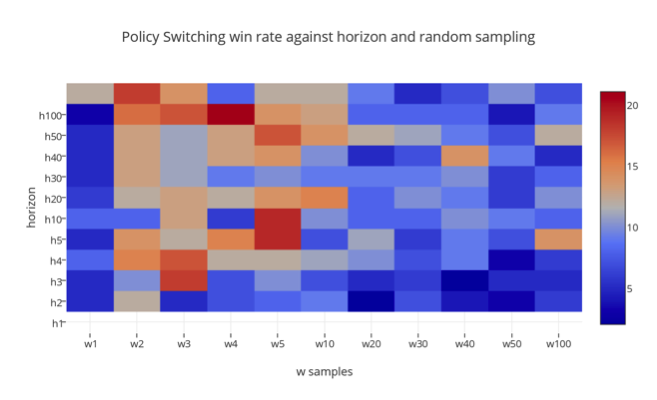
\includegraphics[width=250]{switch.png}
  \caption{number of wins of trials of size 30 vs random policy samples w and horizon h}
\end{figure}
\\
Trials of size 30 were run against an opponent using the BigMoney policy. The kingdom cards were fixed to be: 'Bank','Festival', 'Smithy', 'Library', 'Militia', 'Bazaar', 'Woodcutter', 'Moat', 'Wharf', and 'Throne Room'. Figure 1 shows the number of wins the policy switching player gained out of 30 as w and h increased. The observation that quality is clustered for specific w and h values reinforces our hypothesis that constant toggling of policies isn’t an effective approach, but that there exists a balance and that the parameters w and h can be optimized.
\\
A short test done to verify these results where w, h, and k were evaluated at 1, 2, 5, and 10 where k is the amount of real steps between rollout simulations. We see a similar trend as in the previous results, but clustered more tightly around higher win percentages. Specifically, for those values w and h, the average win rate for k=1 is 17\% while the average win rate for k=10 is 33\%. This leads us to believe that we can also optimize for the amount of time we wait in between rollouts.
\\
\subsection{Offline Policy Search}
\begin{figure}[h]
  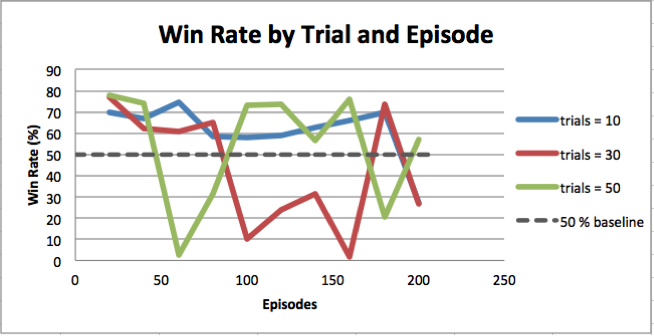
\includegraphics[width=250]{search.png}
  \caption{win rate (\%) by trial and episode}
\end{figure}
\\
In order to evaluate the policy search method, we ran the method with mutation episodes e = [20..200] by 20 and trials t = [10, 30, 50] representing the number of games averaged together to determine the win rate. The resulting policies at the end of all episodes were pitted against the original base policy for 1000 simulated games. The results are shown by the graph in Figure 2. The base policy used for all experiments is shown in Figure 3.
\begin{figure}[h]
  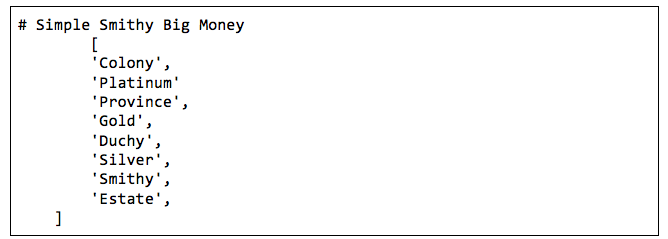
\includegraphics[width=250]{policy.png}
  \caption{base policy}
\end{figure}
The fluctuations in results are due to the fickle nature of the policy representation. Although a single swap in the priority list may seem small, it appears even a single mutation can turn a policy from winning 70\% to 2\% of its games. However, even a bad mutation is occasionally capable of winning enough games by pure luck to beat a better policy, and due to the bootstrapping in the algorithm, this can cause inconsistency and is the likely reason for the large number of very poorly performing outliers.
  \\
  It is curious, since we only accept strict improvements in policies, why it is possible for a policy derived from a base policy could ever be outperformed by its predecessor. It is likely this is also a result of the bootstrapping technique which can result in multiple levels of indirection by the time the final policy is constructed. At the birth of the final policy, its opponent is no longer the base policy, but one that has itself gone through multiple iterations of adaptation. However, in our testing, bootstrapping more than makes up for its inconsistencies in the large boon it provides to the efficiency of the algorithm as well as its introduction of the capacity to run potentially infinite trials as there is no bound on win rate.
  \\
  Despite the frenetic looking graph, the results here are promising. The majority of resulting policies won well over 50\% of their games against the original policy. This bodes well for the future of this or other iterations of this method.
\\
  \subsection{Corollary}
While good for switching on very different policies, when testing the non-trivial policies that are satisfied by common cards, the average total discounted reward for each policy has a very narrow margin in non endgame conditions. This resulted in the toggling we were trying to avoid. We believe this attributed to the large deviation in win rate for policy switching as w grew. As we sampled more policies, in cases where the end condition was outside the horizon of our trajectories, our rewards would be too close and error would become significant. While we still observe that the difference in victory and money between the player and opponent should be rewarded during non-endgame trajectories, a different statistical model will likely improve the algorithm.
\section{Conclusion}
Though the results are not fully conclusive for our online policy search method nor were completely optimize for the parameters of our policy switching approach, they were quite positive and show promise for further experiments. Our goal was not to create the best imaginable Dominion solver, but rather to explore the possibility of Dominion as a domain for MDP style reinforcement learning. We believe we have demonstrated that policy improvement algorithms are highly applicable to the domain of Dominion, and that we have at least provided a basis on which to begin exploring it.
\subsection{Future Work}
  In continuations of this work, we would like to make attempts at a few other methods for policy improvement, including policy gradient. Additionally, there are open areas for improvement in the methods we proposed. We would like to explore other ways to mutate policies for policy search and examine their effects on the algorithm. We expect that the proper additions there may be the key to the potential power of the method.
  \\
  We would like to take one step back and discover a better reward function than the one we reasoned for better incremental improvement. We would like to fix the simulator and derive a better reward function that closely fits known patterns of success when playing dominion, or find non-expert driven ones.
  \\
  Finally, we would be interested in applications of our proposed techniques to other domains. While our implementations are tailored to Dominion in particular, the methods may have applications at the very least to the sizeable set of similar deckbuilding card games and potentially countless other areas. Policy switching has already proven powerful in a number of domains.}
\end{document}
